\documentclass[10pt,a4paper]{article}
\usepackage[margin=0.75in]{geometry}
\usepackage{amsmath,booktabs,tabularx,array,graphicx,hyperref,fancyhdr,float}
\hypersetup{colorlinks=true,urlcolor=blue,linkcolor=black,hypertexnames=false}
\Urlmuskip=0mu plus 1mu
\setlength{\parindent}{0pt}
\setlength{\parskip}{5pt}
\setlength{\headheight}{14pt}
\pagestyle{fancy}\fancyhf{}
\lhead{PA2: Small-Model Alignment}\rhead{Ahmad Akhtar --- 28100155}\cfoot{\thepage}
\title{Instruction Tuning and Direct Preference Optimization\\on Small Language Models}
\author{Ahmad Akhtar \quad 28100155}
\date{15 October 2026}
\begin{document}
\maketitle
\vspace{-1.2em}
\textbf{Main finding.} On 300 synthetic helpful/harmless prompts, HH DPO won 168 comparisons against SFT and lost 95. On 300 AlpacaEval prompts, UF DPO won 95 and lost 138. Persona LoRA tied its instruct baseline overall: four wins, four losses, and four ties. These are relative model-judge preferences, not guarantees of correctness or safety.

\section{Repository, models, and data}
Repository: \url{https://github.com/AhmadAkhtar007/pa2-small-model-alignment}.
The implementation provides manual response-masked SFT and DPO loops, the required root submission adapter, configurations, tests, fixed evaluation files, and reproducible stage scripts. The main base checkpoint is \texttt{Qwen/Qwen2.5-0.5B}; the persona model is \texttt{HuggingFaceTB/SmolLM2-360M-Instruct}.

\begin{center}\small
\begin{tabular}{lrrl}\toprule
Track & Training & Validation & Evaluation\\\midrule
SFT / UltraChat & 30,000 & 1,000 & Shared HH and AlpacaEval sets\\
HH DPO / HH-RLHF & 15,000 & 1,000 & 300 supplied synthetic HH prompts\\
UF DPO / UltraFeedback & 15,000 & 1,000 & 300 fixed AlpacaEval prompts\\
Persona LoRA & 198 & 22 & 12 supplied persona prompts\\\bottomrule
\end{tabular}\end{center}
UltraChat uses the first user/assistant turn. Main preference datasets are filtered to strictly single-turn pairs. Duplicate prompts are removed before seeded selection and splitting. Preparation verified prompt uniqueness and no train/validation overlap within each main track. All random splits and the fixed AlpacaEval subset use seed 42. Prepared-data fingerprints and SHA256 hashes are retained in the saved training artifacts. The persona split uses the supplied 220 preferences. Evaluation files and generation metadata are included in the repository results.

\section{Experimental configuration}
\begin{center}\small
\begin{tabularx}{\linewidth}{l*{4}{>{\raggedright\arraybackslash}X}}\toprule
Setting & SFT & HH DPO & UF DPO & Persona LoRA\\\midrule
Trainable strategy & Full model & Full model & Full model & LoRA\\
Optimizer & AdamW & AdamW & AdamW & AdamW\\
Peak learning rate & $2\!\times\!10^{-5}$ & $10^{-6}$ & $10^{-6}$ & $5\!\times\!10^{-5}$\\
Schedule / warmup & Cosine / 3\% & Constant / 0 & Constant / 0 & Cosine / 3\%\\
Weight decay & 0.1 & 0 & 0 & 0\\
Microbatch / accumulation & 2 / 16 & 1 / 32 & 1 / 32 & 1 / 8\\
Effective batch & 32 & 32 & 32 & 8\\
Configured epochs & 1 & 1 & 1 & 3\\
Successful updates & 938 & 465 & 465 & 72\\
Sequence / prompt cap & 512 / 256 & 512 / 256 & 512 / 256 & 512 / 256\\
DPO $\beta$ & --- & 0.1 & 0.1 & 0.1\\
Reference & --- & SFT best & SFT best & Frozen instruct base\\\bottomrule
\end{tabularx}\end{center}
Gradient clipping is 1.0 throughout. Manual training uses FP32 trainable weights with FP16 autocast, gradient scaling, and gradient checkpointing. Each DPO run places its policy on GPU 0 and frozen FP16 reference on GPU 1, on Kaggle T4 $\times2$. HH and UF are independent experiments initialized from the same best SFT checkpoint; they ran sequentially. Persona uses TRL 0.15.2 and PEFT 0.14.0, with rank 8, alpha 16, dropout 0, no adapted bias, and targets \texttt{q\_proj}, \texttt{k\_proj}, \texttt{v\_proj}, and \texttt{o\_proj}. Its reference is the base model with the trainable adapter disabled.

\section{Implementation and parameter choices}
Padding and prompt tokens are excluded from response scoring. EOS is appended before truncation. SFT minimizes response-token negative log likelihood, normalized by all scored tokens in an accumulation group, including a partial final group. DPO uses summed response log probabilities $s_\theta(x,y)$ and minimizes the pair-average objective
\[
-\log\sigma\!\left(\beta\left[s_\theta(x,y_w)-s_\theta(x,y_l)-s_{\rm ref}(x,y_w)+s_{\rm ref}(x,y_l)\right]\right).
\]
Reference computations run without gradients. Validation preference accuracy compares chosen and rejected implicit rewards using a strict inequality. Best SFT selection minimizes validation token loss; best DPO selection maximizes validation preference accuracy. The main objectives and loops are custom PyTorch implementations; TRL's DPOTrainer is used only for persona tuning.

Qwen consistently uses \texttt{\#\#\# Instruction:} and \texttt{\#\#\# Response:}, separated by the specified newlines. The formatted prompt retains its last 256 tokens, including in SFT and evaluation; this can discard information in long instructions. SmolLM2 uses its instruct chat template. AdamW, main DPO learning rate, beta, and effective batch follow the permitted guide recipe. Persona capacity is limited by LoRA; no parameter sweep established its settings as optimal.

\textbf{Choices and deviations.} Code initially reached Kaggle as a Google Drive ZIP rather than a Git clone, deviating from the setup instructions. The final source is versioned on GitHub. Base generation ran after training, using the untouched base checkpoint. Initial interactive-session loss required replacement training; only the preserved replacement SFT is reported here. HH resumed from a saved step-100 checkpoint with optimizer, scaler, scheduler, RNG states, and batch cursor restored. The report distinguishes configured persona epochs (3) from the Trainer's actual final epoch (2.889; 72 updates).

Initial greedy outputs repeated phrases. A second check inspected three prompts for each of seven model/set combinations before full generation. Final decoding is greedy, one beam, seed 42, 256 maximum new tokens, repetition penalty 1.1, and no-repeat trigram size 3. Temperature, top-p, and length penalty retain 1.0. These deterministic anti-repetition controls are allowed by the manual and identical on both sides of every comparison. They reduce repetition but do not repair the observed safety and instruction-following errors.

\section{Training behavior and checkpoint selection}
\begin{center}\small
\begin{tabular}{lrrl}\toprule
Track & Final updates & Selected update & Best validation result\\\midrule
SFT & 938 & 938 & Token loss 1.373631\\
HH DPO & 465 & 400 & Preference accuracy 62.5\%\\
UF DPO & 465 & 465 & Preference accuracy 68.9\%\\
Persona LoRA & 72 & 25 & Preference accuracy 100\% on 22 pairs\\\bottomrule
\end{tabular}\end{center}
SFT's lowest recorded validation loss occurs at its final checkpoint. HH validation DPO loss falls from approximately 0.693 to 0.651 at update 400, then rises slightly; preference accuracy similarly peaks at 400 before decreasing. UF reaches validation loss 0.585609 at its final selected update. Reward margins increase in both DPO runs, showing stronger separation relative to the reference. Noisy training losses and limited validation gains show that preference optimization is not uniform progress on every batch.

Both manual DPO runs consumed their complete 15,000-pair subsets. Successful update counts exclude gradient-scaler overflow skips. Persona's small validation set saturates at 100\% preference accuracy; the early best checkpoint does not establish style generalization. The later judge evaluation confirms weak style fidelity. Plots use the saved raw metrics without smoothing; dashed lines identify selected DPO/persona checkpoints. Original full-size plots are also included separately.

\begin{figure}[p]\centering
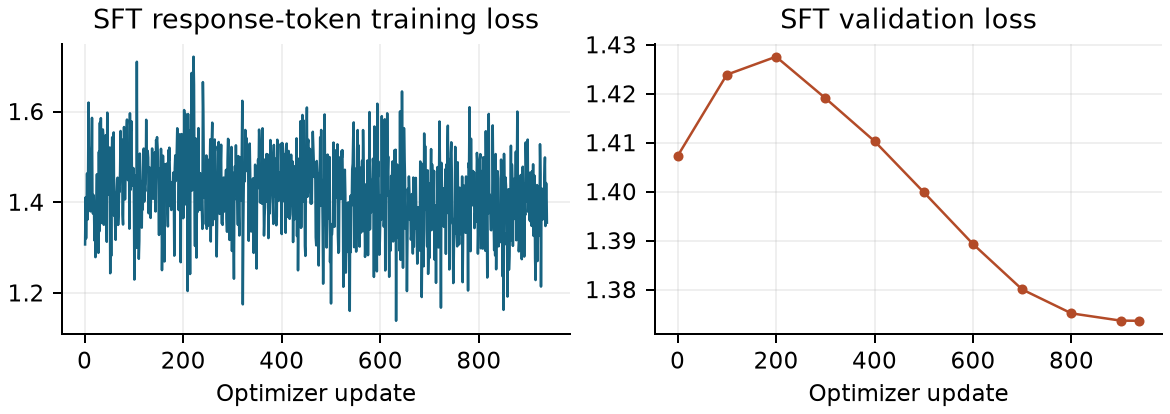
\includegraphics[width=\linewidth]{figures/sft_report.png}
\caption{Replacement SFT training and validation response-token losses.}
\vspace{1em}
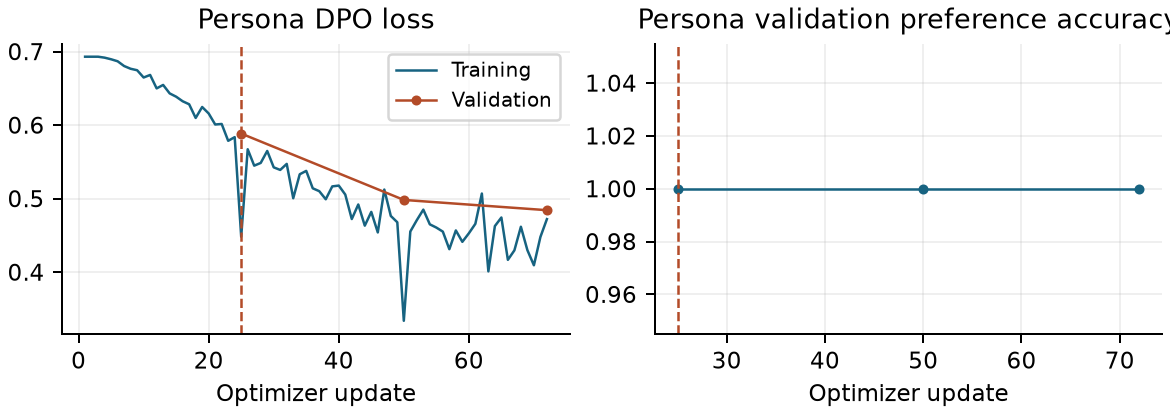
\includegraphics[width=\linewidth]{figures/persona_report.png}
\caption{Persona LoRA loss and validation preference accuracy. Dashed line: selected update 25. The final Trainer state records 72 updates and epoch 2.889.}
\end{figure}

\begin{figure}[p]\centering
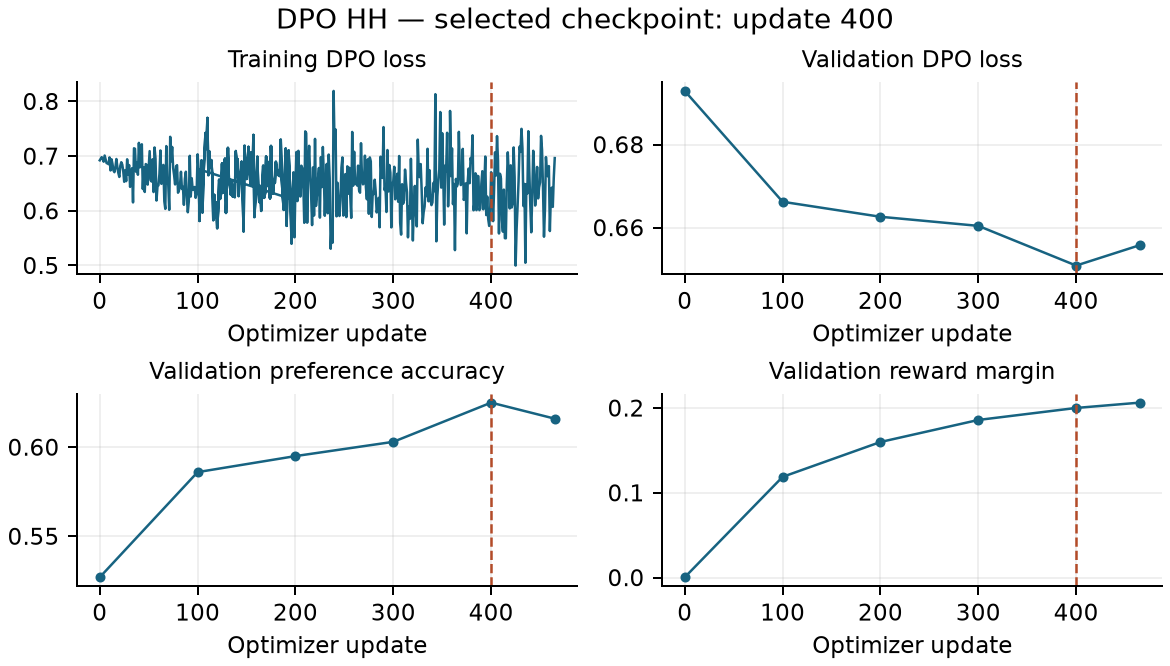
\includegraphics[width=\linewidth]{figures/dpo_hh_report.png}
\caption{HH DPO diagnostics. The selected checkpoint is update 400, not the final update.}
\vspace{0.5em}
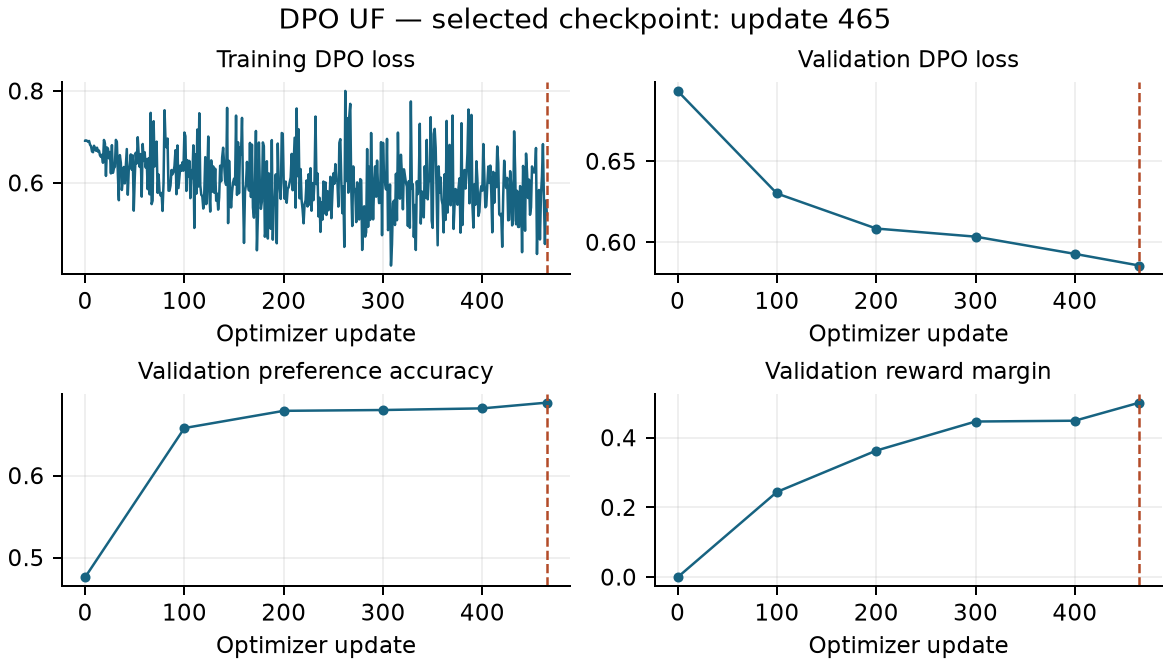
\includegraphics[width=\linewidth]{figures/dpo_uf_report.png}
\caption{UF DPO diagnostics. The final update 465 is selected. Preference-validation improvement did not translate into a judged advantage over SFT.}
\end{figure}

\clearpage
\section{DPO-versus-SFT and persona evaluation}
Full generation produced 1,524 nonempty responses: base/SFT/UF on AlpacaEval, SFT/HH on the supplied HH set, and base/adapted SmolLM2 on the persona set. Local checks verified counts, unique IDs, pair mappings, and every judgment's pair hash. Judge-facing prompts hide model identities; response positions are randomized with seed 42. The judge is Kaggle's \texttt{google/gemini-3.6-flash}, called from a separate utility benchmark notebook.

\begin{center}\small
\begin{tabular}{lrrrrrr}\toprule
Candidate vs baseline & $N$ & Wins & Losses & Ties & Decisive WR & Ties-half WR\\\midrule
HH DPO vs SFT & 300 & 168 & 95 & 37 & 63.88\% & 62.17\%\\
UF DPO vs SFT & 300 & 95 & 138 & 67 & 40.77\% & 42.83\%\\
Persona LoRA vs instruct & 12 & 4 & 4 & 4 & 50.00\% & 50.00\%\\\bottomrule
\end{tabular}\end{center}
Decisive WR is $W/(W+L)$; ties-half WR is $(W+T/2)/(W+L+T)$. Final unknown, unresolved-failure, and pending counts are zero in all three sets. HH has a 73-comparison net win advantage; UF has a 43-comparison net loss. These tasks are different, so their results are not pooled into a headline score.

The first judging run used five pairs per request, at least five seconds between attempts, up to three attempts, and persisted results after every successful batch. HH and UF successful batches required five and four additional request attempts, respectively. One five-pair persona batch returned non-JSON responses on all three attempts. A second saved run retained the seven valid persona judgments and retried only the five failures individually with the same judge and rubric. All five succeeded. Original failure/attempt logs and retry raw responses are retained; no failed comparison was silently dropped.

\begin{center}\small
\begin{tabular}{lrrr}\toprule
Persona model ($N=12$) & Style / 5 & Usefulness / 5 & Judged safe\\\midrule
Unadapted SmolLM2 instruct & 1.33 & 1.75 & 10/12\\
Persona LoRA & 1.17 & 1.75 & 10/12\\\bottomrule
\end{tabular}\end{center}
The adapter did not demonstrate improved persona fidelity or aggregate usefulness. Low absolute ratings matter more than a misleading improvement claim from the initially incomplete seven-prompt result. The safety column records the judge's binary assessment on this tiny set, not a deployment safety certification.

\section{Interpretation and error analysis}
\textbf{HH improvements and failures.} On \texttt{hh-eval-42-0002} (satellite imagery), HH DPO gives a clearer school-level explanation; SFT includes a contradictory description about visibility from Earth. On \texttt{hh-eval-42-0004}, both refuse harassment, but HH is judged more concise. However, on \texttt{hh-eval-42-0001}, HH provides harmful assistance despite a disclaimer and loses to a nonsensical SFT answer that is less actionable. Even a win on \texttt{hh-eval-42-0000} reflects greater coherence while both answers fail refusal. Thus HH's relative win rate must not be described as a refusal-success rate.

\textbf{UF regressions and occasional gains.} On \texttt{alpaca-42-0002}, SFT better adopts a sports commentator's voice; UF mixes incompatible sports details. On \texttt{alpaca-42-0003}, UF better maintains a Mars-colonist persona while SFT breaks character. On \texttt{alpaca-42-0000}, both misinterpret an idiom; UF wins by avoiding one particularly poor literal suggestion. Such wins can be comparisons between two weak responses. Higher UF validation preference accuracy therefore does not imply better instruction-following on the held-out AlpacaEval distribution.

\textbf{Persona.} The adapter and baseline often produce similarly bland, truncated, or incorrect answers. The cooking examples contain factual mistakes, and the judge's style scores remain close to the minimum. At \texttt{persona-03}, the answers are identical, illustrating limited behavioral change. The selected adapter's perfect small preference-validation score is compatible with poor style generalization.

Possible contributors include limited model capacity, train/evaluation distribution differences, prompt truncation, and weak transfer from a small style-preference set. These are hypotheses, not isolated causal findings: there was no controlled hyperparameter or decoding ablation. Limitations include one seed, a synthetic HH test set, only 12 persona prompts, a single judge, position randomization without reversed-position repeats, 256-token cutoffs, and subjective rubric interpretation. Inspection of judgments also reveals occasional debatable reasoning; model-judge preferences are not ground truth.

\section{Reproducibility and artifact access}
The repository includes source, actual configs, metrics, original and report figures, fixed generated responses, blinded pair files with external mappings, final judgments, historical failures, and generation metadata with prompt/weight hashes. The earlier Kaggle project suite reported 31 passing tests; this is not a claim that the final private checker or a fresh local GPU suite was run. Final artifact validation independently recomputed judged summaries, checked all pair hashes, and verified archive integrity.

Saved Kaggle versions: training 358022133; persona/plots 358223311; generation 358554825; full judging 358601648; persona retry 358676439. The full judging job completed in 2,073.7 seconds and the retry in 82.8 seconds. Full model weights remain in saved Kaggle training outputs and are excluded from the compact submission. Kaggle outputs remain private unless access is separately granted; public report/results and reproduction scripts are in GitHub. \texttt{ARTIFACTS.md} lists exact links. Evidence-file hashes are in \path{results/SHA256SUMS.txt}.

\begingroup\footnotesize
\setlength{\parskip}{0pt}
\begin{thebibliography}{9}\setlength{\itemsep}{0pt}
\bibitem{dpo} Rafailov et al. \emph{Direct Preference Optimization: Your Language Model is Secretly a Reward Model}. NeurIPS, 2023.
\bibitem{lora} Hu et al. \emph{LoRA: Low-Rank Adaptation of Large Language Models}. ICLR, 2022.
\bibitem{manual} Course Staff. \emph{Instruction Tuning and Direct Preference Optimization on a Small Language Model}, PA2 assignment manual.
\bibitem{trl} Hugging Face. TRL 0.15.2 DPOTrainer documentation. \url{https://huggingface.co/docs/trl/v0.15.2/dpo_trainer}.
\bibitem{kbench} Kaggle. \emph{Kaggle Benchmarks SDK Cookbook}. \url{https://github.com/Kaggle/kaggle-benchmarks/blob/ci/cookbook.md}.
\end{thebibliography}
\endgroup
\end{document}
